\begin{figure}[t]
\centering
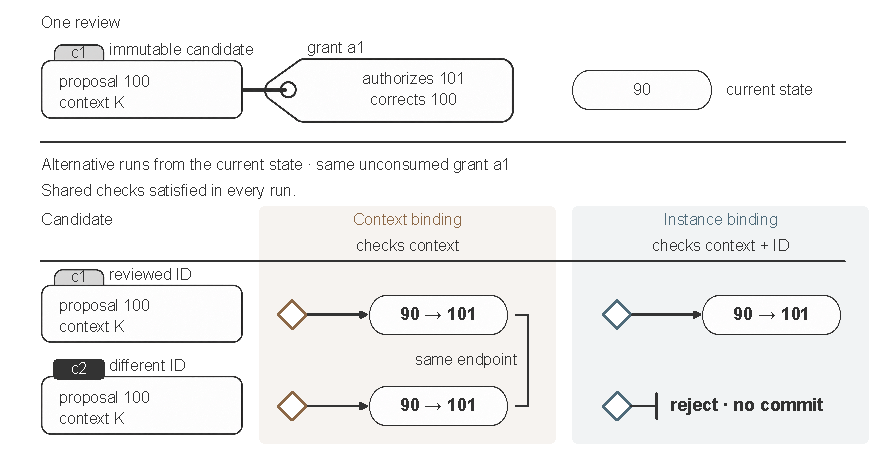
\includegraphics[width=\linewidth]{figures/fig1-review-execution-gap.pdf}
\caption{Equal endpoints do not identify the reviewed instance. A reviewer corrects candidate c1's proposal 100, and grant a1 authorizes 101 for c1. Candidate c2 carries the same proposal and retained context $K$ but a different identifier. Each path represents an alternative execution from the current state 90 with the original grant a1 still unconsumed and the shared checks satisfied. Diamonds mark checks, capsules show the initial state or committed transitions, and the stop bar marks no commit. Context binding admits either candidate and installs 101; instance binding admits only c1. A matching new authorization could license c2, subject to the shared checks. The four roles are the machine proposal (100), the authorized correction (101), the reviewed candidate (c1), and the executed transition ($90 \to 101$). This is a conceptual construction. Object glyphs were AI-generated; see the AI-assisted preparation declaration}
\label{fig:gap}
\end{figure}


\section{Introduction}\label{introduction}

Gerrit's \texttt{copyCondition} determines whether a code-review vote carries forward to a new patch set \citep{gerrit-copy-condition}. Agent software faces the same decision when a reviewed update is regenerated or crosses a queued handoff: which replacements may reuse approval? Human-in-the-loop middleware supports approval, argument edits, rejection and resumption \citep{langchain-hitl}; the application must still relate its persisted grant to the candidate eventually written.

Consider persisted candidates c1 and c2 with the same proposal 100, evidence, producer and expected predecessor, but different identifiers. A reviewer inspects c1 and authorizes 101; a later handoff supplies c2 under that grant and installs 101. Value, predecessor and retained-context checks pass, yet execution uses a different candidate. This is the \textbf{review--execution gap}. A policy permitting equivalent candidates can accept c2; one attaching responsibility to the reviewed artifact must preserve c1's identity. Endpoint correctness does not imply continuity of the reviewed candidate.

We characterize this choice with a four-role contract linking the machine proposal, authorized correction, reviewed candidate and persisted transition. Context binding accepts candidates with equivalent retained review information; instance binding additionally requires the reviewed instance. Both share authorized-value equality, predecessor freshness, an atomic complete successor and field-source preservation. Paired execution from the same review checkpoint isolates the instance requirement from the agent's response.

Our design space organizes which review object to retain, which relationships to check before writing and which continuation a failed check should expose. Store implementations and independent persistence checks connect these choices to durable effects; an external-framework study maps the obligations to existing extension interfaces.

Two comparisons separate approval coverage from continuation cost. Nine constructed cases distinguish omitted-field changes, content-equivalent replacements and mutable external dependencies. The paired agent study holds retained content fixed ($K=R$) and measures recovery after identity-only rejection, rather than the benefit of preventing semantic change. Native LangChain and LangGraph probes locate the boundary between interrupt approval and application-level binding of a persisted business grant.

For builders of agentic software, the paper makes four contributions (Table~\ref{tab:evidence-map}):

\begin{enumerate}
\def\labelenumi{\arabic{enumi}.}
\tightlist
\item
  \textbf{A comparison of approval-binding design choices.} We organize value, context, content and instance binding under shared checks, nested compared fields and immutable records, and expose their boundaries in nine constructed cases.
\item
  \textbf{Measured agent continuation under an instance requirement.} Paired execution isolates instance equality; event-order analysis separates recovery commits, subsequent confirmation and complete paired-suffix cost.
\item
  \textbf{An explicit contract for corrected execution.} Value, freshness, successor and source obligations connect the four roles. A constructive result shows why equal predecessors and final values do not determine review continuity.
\item
  \textbf{Executable enforcement and persistence-based validation.} Store implementations, controlled cases, bounded Alloy checks and an independent auditor validate durable effects. A ToolGate adaptation combines normal callbacks with an author-written commit bridge on public reference workflows.
\end{enumerate}

\begin{table}[tbp]
\caption{Contributions and their principal evidence.}\label{tab:evidence-map}
\centering\small
\begin{tabularx}{\textwidth}{@{}>{\raggedright\arraybackslash}p{0.40\textwidth}>{\raggedright\arraybackslash}p{0.42\textwidth}>{\raggedright\arraybackslash}X@{}}
\toprule
Contribution & Principal evidence & Section \\
\midrule
1. Compare binding choices & Nine constructed comparator cases; conditional inclusion & \ref{binding-scope-and-native-defaults} \\
2. Characterize continuation & Frozen paired suffixes; recovery event order & \ref{two-routes-to-accountable-recovery} \\
3. Specify the correction relation & Fixed-registry witness; local observation model & \ref{what-endpoint-correctness-cannot-establish} \\
4. Realize and validate obligations & Store checks; external ToolGate adaptation & \ref{realization-and-external-comparison} \\
\bottomrule
\end{tabularx}
\end{table}

\section{Related Work}\label{related-work}

\subsection{What existing mechanisms bind}\label{existing-binding-and-enforcement-mechanisms}

Existing mechanisms bind authority to different objects: an interrupted call, patch set, saved plan, sealed proposal, commit-time witness or symbolic-state predicate (Table \ref{tab:related}). Code review makes applicability configurable through vote copying, approval reset and submit requirements \citep{gerrit-copy-condition,gitlab-approvals}. We study that choice for corrected agent state and its consequences for continuation.

\begin{table}[tbp]
\caption{Binding, mismatch handling and evidence in the cited sources. The two attack analyses describe failure paths; their check points are observation points.}\label{tab:related}
\centering\footnotesize
\setlength{\tabcolsep}{2.5pt}
\renewcommand{\arraystretch}{1.05}
\begin{tabularx}{\textwidth}{@{}>{\hsize=1.05\hsize\raggedright\arraybackslash}X>{\hsize=1.0\hsize\raggedright\arraybackslash}X>{\hsize=1.05\hsize\raggedright\arraybackslash}X>{\hsize=.75\hsize\raggedright\arraybackslash}X>{\hsize=1.15\hsize\raggedright\arraybackslash}X@{}}
\toprule
Mechanism & Binding object & Mismatch handling & Check point & Evaluation form \\
\midrule
LangChain HITL \citep{langchain-hitl} & Interrupted tool call & Reviewer may edit/reject, then resume & Before tool execution & Interface documentation \\
ReSA \citep{zhu2026resa} & Grant scope; consumed versions & Derive repair obligations & Reconstruction to local sink & Authored graphs; installed-control checks \\
Guarded Commits \citep{bindschaedler2026guarded} & Artifact, policy; edit hashes & Fresh authorization or review & Commit & Public-trace replay; synthetic DAGs \\
Cordon \citep{cordon} & Task, lineage, staged effects & Abort, rollback, compensation & Commit or effect release & Agent workflows; scripted rollback/resume \\
Continuity Kernel \citep{continuity-kernel} & Proposal ID; sealed successor & Reject, quarantine or defer; new-ID retry & Atomic activation & Bounded model exploration \\
Commit-time authorization \citep{commit-time-auth} & Witness, target, eligibility & Abort or refresh/rebind & Durable-effect boundary & Agent perturbations; replay; limited enforcement \\
ToolGate \citep{toolgate} & Symbolic state; tool contracts & Filter call; discard invalid result & Tool invocation; state update & ToolBench; MCP-Universe \\
Gerrit / GitLab \citep{gerrit-copy-condition,gerrit-submit-requirements,gitlab-approvals} & Patch set / merge request & Copy or reset votes by policy & New revision; submit/merge & Product documentation \\
OpenTofu \citep{opentofu-plan-apply} & Saved plan decisions & Plan mismatch: not assessed in cited guide & Plan application & Command documentation \\
\midrule
Loopjacking \citep{kumar2026loopjacking} & Analyzed: call identity and arguments & Substitution attack; deny-update control & Review, update, resume & Released Agno; configured LangGraph tests \\
Approval Laundering \citep{wang2026approval} & Analyzed: grant, dispatch, effects & Policy divergence; token-replay check & Dispatch; effect sinks & Claude Code probes under research policies \\
\midrule
This work & Compared: context, content and instance & Reuse reviewed instance or reauthorize & Atomic successor write & Formal/store checks; paired agent continuation \\
\bottomrule
\end{tabularx}
\end{table}


ReSA derives approval-scope repair obligations from consumed versions, trusted preservation and atomic validation \citep{zhu2026resa}. Guarded Commits checks path coverage and pinned policy, binds EDIT decisions to pre-edit, delta and post-edit hashes, and creates a fresh record for valid decision reuse \citep{bindschaedler2026guarded}. Our correction relation organizes the machine proposal, authorized correction, reviewed candidate and installed transition with field-source preservation. Holding context, authorized values, freshness and persistence checks fixed, we compare whether approval covers a content-equivalent candidate or only the reviewed instance, then measure agent recovery and cost.

Continuity Kernel seals proposal identity and exact candidates through atomic activation. Commit-time authorization distinguishes endpoint success from valid authority at durability and includes recovery comparisons \citep{commit-time-auth}. Cordon studies workflow execution and approval costs. These mechanisms supply foundations for our controlled binding comparison; ToolGate's application pre/postconditions provide an external implementation target (Section \ref{configured-toolgate-on-public-reference-workflows}).

Loopjacking exposes changed tool arguments executing under a review of different arguments in Agno and a LangGraph Agent Server composition \citep{kumar2026loopjacking}. Approval Laundering examines divergence between approved invocations and dispatched actions or downstream effects in Claude Code \citep{wang2026approval}. Our paired study examines the complementary identity-only case: correction and retained context remain equal, and the selected binding rule determines whether the agent must recover.

\subsection{Foundations and the correction relation}\label{foundations-and-the-correction-relation}

Transactions and concurrency control supply atomicity and predecessor validation \citep{gray-transaction,kung-occ}. Provenance covers derivations, edits and copies \citep{buneman-provenance,cheney-provenance,buneman-curated}, transaction reenactment \citep{arab-reenactment} and entity/activity/agent descriptions \citep{prov-dm}. Interactive repair separates machine suggestions from human judgments \citep{yakout-guided-repair,falcon-cleaning}. Our contract joins these concerns in the installed successor's authorized correction, reviewed-candidate link and field sources.

Integrity and capability systems connect principals, permitted operations and protected objects \citep{clark-wilson,hardy-confused-deputy,miller-robust-composition}. Runtime verification and monitoring address execution conformance and enforceable policies \citep{runtime-verification,policy-enforcement}; information-flow control constrains propagation \citep{ifc}, and accountability supports reconstructible, attributable execution \citep{accountability}.

Table~\ref{tab:obligation-positioning} maps the obligations defined below to their existing foundations and their role in this study. This composition separates three diagnostic questions: whether the old grant covers the submitted candidate, whether the transition uses the reviewed instance, and whether the successor preserves the required field sources. The agent study then observes continuation after rejection under the instance rule, separating recovery commits from later confirmation. These connected questions and observations define our increment over the reused mechanisms; the table does not claim that the cited systems cannot express these relations.

\begin{table}[tbp]
\caption{Existing foundations and their role in the corrected-execution comparison. P1--P6 are defined in Section~\ref{admission-and-persistence}.}\label{tab:obligation-positioning}
\centering\small
\begin{tabularx}{\textwidth}{@{}>{\raggedright\arraybackslash}p{0.12\textwidth}>{\raggedright\arraybackslash}p{0.37\textwidth}>{\raggedright\arraybackslash}X@{}}
\toprule
Obligation & Existing basis & Role in this study \\
\midrule
P1 & Continuity Kernel binds proposal and sealed candidate; ReSA tracks the consumed object \citep{continuity-kernel,zhu2026resa}. & Vary reviewed-instance equality while holding the correction and shared checks fixed; observe continuation. \\
P2 & ReSA requires preserved or atomically validated consumed versions \citep{zhu2026resa}. & Compare retained context and declared content; separate external referent checks. \\
P3 & Guarded Commits binds authority and pre-edit, delta and post-edit hashes \citep{bindschaedler2026guarded}. & Retain the machine proposal separately from the authorized correction and committed value. \\
P4 & Optimistic concurrency control and Continuity Kernel validate predecessors \citep{kung-occ,continuity-kernel}. & Keep freshness shared across policies, separate from instance mismatch. \\
P5 & Transactions and Continuity Kernel install an atomic accepted unit \citep{gray-transaction,continuity-kernel}. & Install the complete corrected successor, sources, transitions and grant consumption together. \\
P6 & Provenance and curated-database copying retain derivation and source relations \citep{buneman-provenance,buneman-curated}. & Link changed fields to authorized transitions and copy unchanged fields' exact prior sources; check these relations in persistence. \\
\bottomrule
\end{tabularx}
\end{table}


\section{A Contract for Corrected Execution}\label{a-contract-for-corrected-execution}

\subsection{Four roles}\label{four-roles}

Figure \ref{fig:gap} illustrates the four roles: proposal 100, authorized correction 101, reviewed candidate c1 and the transition from 90 to 101.

A persisted candidate is

\[
c = \langle \operatorname{id}, r, f, e, v_{\mathrm{exp}}, x_c, p\rangle
\]

where \(\operatorname{id}\) names a content-immutable persisted candidate record, \((r,f)\) the record and field, \(e\) the evidence and locator, \(v_{\mathrm{exp}}\) the expected predecessor, \(x_c\) the proposal, and \(p\) the producer. An authorization \(a = \langle c_r, x_a, q\rangle\) records the reviewed candidate, explicitly authorized value and authorized principal. Execution submits candidate \(c_s\) and value \(x\), producing a persistent transition. These elements define the four roles: the \textbf{machine proposal}, the \textbf{authorized correction}, the \textbf{reviewed candidate} and the \textbf{executed transition}. The proposal remains in the record when correction makes \(x_c \ne _{\mathrm{json}} x_a\); the successor must contain \(x_a\).

Retained context \(K(c)\) comprises record and field, evidence identity and locator, expected predecessor, proposal and producer. Candidates are \emph{context-equivalent} when they agree on \(K\), and \emph{content-equivalent} when they agree on declared fields \(R\supseteq K\), under the specified comparator. \emph{Same-semantics} means the same approved effect under the scenario oracle. An \emph{identity-only substitution} preserves the declared tuple's non-identifier components while changing its identifier. Instance-creation and outer envelope metadata lie outside this tuple. Value comparisons use canonical JSON equality.

\subsection{Admission and persistence}\label{admission-and-persistence}

Define context and identity agreement by

\[
K_{\mathrm{eq}} \Leftrightarrow  K(c_s) = K(c_r),   I_{\mathrm{eq}} \Leftrightarrow  \operatorname{id}(c_s) = \operatorname{id}(c_r)
\]

Let \(G\) collect the shared checks: valid authority and grant, context/evidence integrity, authorized-value equality, current predecessor, complete successor, source relations and transaction constraints. The integrity component of \(G\) concerns whether the submitted candidate is internally consistent with its evidence; it is separate from \(K_{\mathrm{eq}}\), which compares the submitted and reviewed contexts. The two policies are

\[
P_{\mathrm{context}}: \operatorname{Admit} = G \land  K_{\mathrm{eq}}
\] \[
P_{\mathrm{bound}}:   \operatorname{Admit} = G \land  K_{\mathrm{eq}} \land  I_{\mathrm{eq}}
\]

Both policies retain the reviewed identifier in the authorization; they differ only in the execution rule. Context binding treats the retained information as the approval object; instance binding attaches responsibility to the reviewed artifact. A same-key retry retrieves the existing result, whereas re-preview can materialize a new candidate requiring a matching grant.

The execution contract combines six obligations: \textbf{P1}, instance binding under the bound policy; \textbf{P2}, context and evidence integrity; \textbf{P3}, principal authority and the authorized value; \textbf{P4}, predecessor freshness; \textbf{P5}, one complete atomic successor; and \textbf{P6}, field-source relations. Changed fields point to their authorized transitions; unchanged fields retain their exact prior sources. The successor, transitions, sources and grant consumption commit atomically. Direct-write exclusion (P0) places all authoritative mutation behind this boundary.

Trusted candidate storage is a separate prerequisite: a candidate identifier must resolve to one content-immutable record, and the executor must consume that record. Candidate creation does not confer permission to overwrite an existing candidate or its review linkage. P0 excludes bypass writes to authoritative state; it does not by itself establish this storage prerequisite. External referents require the separate consumption check in Section~\ref{binding-scope-and-native-defaults}.

\subsection{What endpoint correctness cannot establish}\label{what-endpoint-correctness-cannot-establish}

The exact policy difference is the request-state set

\[
S = \{r : G(r) \land  K_{\mathrm{eq}}(r) \land  \neg I_{\mathrm{eq}}(r)\}
\]

so bound admission refines context admission. The following witness illustrates what endpoint checks leave unresolved.

\textbf{Endpoint indistinguishability.} \emph{Equal predecessor states and equal final values can carry different review continuity.} Take independent copies of the same pre-admission state and unconsumed grant. In one copy, context binding admits \((c_s,x_a)\); in the other, instance binding admits \((c_r,x_a)\). When the candidates differ only in identity, both successors have the same field-wise values and copied sources, but only the second transition uses the reviewed instance. The archived fixed-registry witness isolates this difference while holding the other observations fixed. Because the two executions also agree on retained context, a check that reads only final values, predecessor freshness and retained context assigns both the same verdict; continuity must be observed through the candidate--authorization binding itself.

With authorization parameters fixed, five information classes suffice for the declared local classification: candidate--authorization binding, role-labeled values, predecessor discriminators, successor structure and field sources. Online Resource 2, A9 defines the classification and gives witness pairs establishing irredundancy; Online Resource 1, S2 supplies executable checks.

Gate soundness is conditional on direct-write exclusion, a trusted gate and adapter, authority checked at commit entry, consistent equality, transaction-scoped reload and predecessor validation, and atomic installation of the checked relations. Under these premises, a bound commit satisfies the locally checked obligations (P1--P5 and the declared local source checks). Full trace soundness (P6) additionally requires a trace-complete predecessor, immutable valid references, validated new chain links and uniqueness of the successor's transitions; this extension is supported by bounded preservation checks and audits rather than by a general proof. Conversely, a nonempty change that satisfies the remaining contract conditions is accepted when the gate observes the authoritative state and its grant and key remain usable; the detailed acceptance conditions are in A9.

\subsection{Continuation after rejection}\label{continuation-after-rejection}

For an identity-only mismatch, the agent can reuse the reviewed candidate under its still-valid grant or obtain/use a matching authorization for another candidate. Changed evidence or a stale predecessor requires a new candidate reflecting current state and matching authorization. A consumed grant with a prior commit instead calls for receipt retrieval or state confirmation. Each new admission must satisfy the remaining checks.

A rejection thus identifies the failed relationship, and the continuation shows whether an agent can restore it. Section \ref{paired-agent-execution} measures those subsequent actions and their cost.

\section{A Design Space for Binding Review to Execution}\label{design-space}

The contract makes the approval object an explicit engineering choice. If responsibility attaches to a reviewed artifact, instance binding preserves that relationship even when final values agree. If the application permits interchangeable candidates, context binding expresses that rule. Under immutable records and shared checks, stronger binding narrows admission; reauthorization instead changes the continuation branch. API-specific comparison semantics remain essential \citep{rfc9396}.

Three axes organize this choice (Figure \ref{fig:design}). The first is the binding object: no gate, value, context, content or instance. Under trusted lookup of content-immutable records, identity equality implies content equality and hence context equality. Writing \(P_{\mathrm{value}}=G\), and defining content binding on fields \(R\supseteq K\), gives \(P_{\mathrm{bound}} \subseteq P_{\mathrm{content}} \subseteq P_{\mathrm{context}} \subseteq P_{\mathrm{value}}\) under shared checks. Thus \(K_{\mathrm{eq}}\) is redundant under instance binding. The adapter must preserve the resolved immutable record to use: the trusted-preservation case of ReSA \citep{zhu2026resa}, with external documents checked separately at consumption. The contract and online G handoff use \(K=R\) over the declared non-identifier fields, excluding outer host metadata; the levels separate when retained context omits a decision-relevant field (Section \ref{binding-scope-and-native-defaults}).

The second axis is mismatch handling: adoption with a substitution record, unexplained denial, actionable rejection or routing to reauthorization. The tested context policy adopts the substitute and records its identifier. Reauthorization is a continuation branch, not another binding level: it retains the instance decision at admission but provides a matching new grant. The third axis is the check's anchor and timing: request, server-held review record or persisted constraint, checked at review, handoff, commit or grant consumption.

\begin{figure}[tbp]
\centering
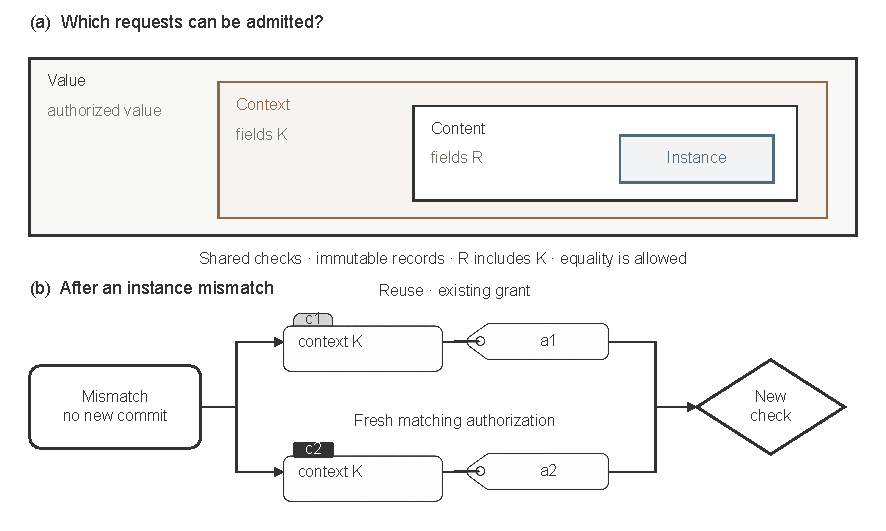
\includegraphics[width=\linewidth]{figures/fig3-design-space.pdf}
\caption{Binding and recovery are separate design choices. Under shared checks and content-immutable candidate records, if the compared content fields \(R\) include the retained context fields \(K\), the admissible request sets satisfy \(A_{\mathrm{instance}}\subseteq A_{\mathrm{content}}\subseteq A_{\mathrm{context}}\subseteq A_{\mathrm{value}}\). These inclusions need not be strict; context and content binding coincide when \(K=R\). Following an instance-mismatch rejection, the system may offer reuse of the reviewed candidate under the existing authorization or obtain matching authorization for another candidate. Reauthorization is a recovery branch, not another binding level. Each continuation must pass a new admission check; the schematic does not guarantee that an available route will be taken. Object glyphs were AI-generated; see the AI-assisted preparation declaration}
\label{fig:design}
\end{figure}


Online Resource 2, A10 maps responsibility rules, compared fields, trusted persistence and continuation to implementation choices. Section \ref{binding-scope-and-native-defaults} compares three binding rules deterministically; Section \ref{paired-agent-execution} tests agents under context binding with recorded substitution and instance binding with a continuation channel. The remaining combinations are design options.

\paragraph*{Two responsibility choices.}
Consider a design example: a release reviewer corrects a configuration in an immutable change record, and the owner requires the installed transition to name that record. Rebuilding identical content preserves the effect but loses this link. Recording the substitution does not authorize approval transfer; reuse under the valid grant or authorization for the replacement preserves the rule. Alternatively, the owner may permit carryover whenever the complete configuration, evidence and predecessor agree. Content binding with a recorded substitution then suffices. Gerrit's configurable vote copying illustrates such explicit project policy \citep{gerrit-copy-condition}. The owner's responsibility rule therefore determines the binding and recovery choices.

\section{Realization and External Comparison}\label{realization-and-external-comparison}

\subsection{Execution gate and independent checks}\label{execution-gate-and-independent-checks}

The contract runs in a relational store and an event journal. The relational adapter reloads state, evidence and authorization within the transaction, validates the principal and unused identities, compares-and-swaps the predecessor, and installs the complete successor, transitions and exact sources. The journal records the same relations under context and exact configurations differing only in instance equality. An independent database oracle reads persisted pre/post relations; a source verifier follows field links through transitions, authorizations, candidates, evidence and predecessors.

The controlled suite runs 165 cases per mechanism. The context journal accepts 60 and rejects 105; the exact journal and relational reference each accept 45 and reject 120. The 15 differences are same-context substitutions. The two exact implementations also agree on provenance-query answers. Request/display probes and the case mapping appear in Online Resource 2, A6.

Bounded formal checks and a historical audit support the same relations. Alloy/Kodkod checks \citep{alloy,kodkod} cover admissions, conjunct removal, source attacks and trace preservation: 72 command outcomes match the manifests, with no assertion counterexamples in the encoded finite scopes. The independent mapping has nine intended satisfiable projections and twenty unsatisfiable mutants. A historical audit reconstructs 84 machine-origin correction chains from 1,260 hosted databases, checking 252 evidence associations, 168 record versions and 168 provenance traces. It establishes that the four roles can be recovered from the retained persistence records; unchanged-field copying is exercised in the controlled multi-field cases (Online Resource 1; Online Resource 2, A5--A6).

\subsection{ToolGate portability case study}\label{configured-toolgate-on-public-reference-workflows}

ToolGate \citep{toolgate} supplies symbolic state and application pre/postconditions. Its normal callbacks express the binding, value, predecessor and source obligations; an author-written SQLite bridge supplies the record schema and durable commit boundary. This tests implementability through extension interfaces, not native default admission.

Execution has four stages: callbacks check the request; the native tool drafts changes in a cloned world; postconditions validate the draft; the bridge installs the successor and its relations in SQLite. Persisted state is then projected back into the public world for the reference suffix (Online Resource 2, A8).

Both implementations pass eight development controls. Six public Retail workflows from the pinned tau2-bench repository \citep{tau2-bench}, crossed with four scenarios, yield 24 routes per implementation (Table \ref{tab:external}). Both satisfy the shared business checks and scripted recovery. ToolGate's one strict failure is two initialization log lines violating the empty-output rule; the frozen failure is retained separately from business-state scores. Scripted decisions establish implementability on these workflows (Online Resource 2, A8).


\begin{table}[tbp]
\caption{Configured ToolGate ($T$) versus the contract backend ($C$). Development controls and public workflow routes are separate units; decisions and recovery are scripted.}
\label{tab:external}
\centering\small
\begin{tabularx}{\textwidth}{@{}Xrr@{}}
\toprule
Check & $T$ & $C$ \\
\midrule
Development controls satisfied & 8/8 & 8/8 \\
Public: initial authorized business commits & 12/12 & 12/12 \\
Public: invalid requests rejected without a business write & 12/12 & 12/12 \\
Public: fixed legal recovery commits & 12/12 & 12/12 \\
Public: complete reference-world matches & 24/24 & 24/24 \\
Public: frozen strict PASS/FAIL & 23/1 & 24/0 \\
\bottomrule
\end{tabularx}
\par\smallskip
\begin{minipage}{\textwidth}\small
Six public workflows crossed with four controlled scenarios give 24 routes per implementation.
The retained strict failure is two initialization log lines violating an empty-output rule.
Post-hoc inspection confirms that route's business relations and final reference world;
the frozen FAIL is unchanged. Reference-world agreement is not an official benchmark
success rate or evidence of autonomous recovery.
\end{minipage}
\end{table}


\subsection{Binding scope and native defaults}\label{binding-scope-and-native-defaults}

Two deterministic experiments characterize resume routing and the fields each binding comparator checks. Neither calls a model. Online Resource 2, A11 identifies the protocol, saved runs and reproduction commands.

\textbf{Native human-in-the-loop defaults.} We test unmodified LangChain middleware \citep{langchain-hitl} and the LangGraph interrupt primitive (langchain 1.2.10, langgraph 1.0.8) with an author-written graph, executor, recorder and primitive payload schema. Sixteen deterministic conditions record 18 SQLite effects. Two-turn conditions retain one graph, checkpointer and thread. In both mechanisms, a second turn creates a new interrupt without writing. Resuming with the earlier identifier leaves approval pending and adds no write; the current identifier permits one. Repeating affirmative input at the new interrupt also writes once, constituting fresh approval rather than reuse. An explicit edit from 100 to 999 persists 999 while earlier checkpoints retain the original proposal and review payload; malformed middleware decisions raise errors without writing. Thus approval addresses the pending interrupt, and no earlier approval was consumed by a later request in these routes. Binding a persisted business grant remains an application decision. The probe covers successive interrupts and edits, not same-identifier pending-call replacement or Loopjacking's Agent Server configurations \citep{kumar2026loopjacking}.

\textbf{Binding scope.} Nine constructed cases cross three binding comparators and a diagnostic variant with two execution modes, giving 72 routes (54 principal, 18 diagnostic). All arms apply the same authorized-value guard and differ only in the compared fields (Table \ref{tab:binding-scope}). In one case the reviewed document changes after review while the candidate stays identical, and a matched control leaves it unchanged. An unchecked executor reads the live document; a verifying executor checks the reviewed digest and consumes the same captured bytes, stopping on mismatch. An independent scorer reads only the persisted effects and compares them with the approved effects saved before execution; it detects deliberate deletion, addition and alteration in copies of each sink.

This experiment uses an extended candidate schema: $K$ contains the target record, operation, unit, source-document digest and proposal; $R$ adds effective date and cost center. A note enters both projections only when declared semantic. Monetary values are normalized to two decimal places. These comparators and the common executor test binding scope, not the full shared gate $G$. In contrast, the contract's declared tuple and the online G handoff use $K=R$ with canonical JSON equality.

% Generated by scripts/figures/build_binding_matrix.py
% FIGURE-DATA.json SHA256: 3a639de0cbd7b11b757ccb84f788dfef3c21ade0fdf660ecaec4792bb0fab6c5
\begin{table}[tbp]
\caption{Binding-gate decisions over nine constructed cases. A: admit; R: reject. Each decision is identical under unchecked and verified execution (72 routes); entries do not report writes. All comparators share the authorized-value check.}\label{tab:binding-scope}
\centering\footnotesize
\setlength{\tabcolsep}{3pt}
\renewcommand{\arraystretch}{1.12}
\begin{tabularx}{\textwidth}{@{}>{\raggedright\arraybackslash}p{0.46\textwidth}*{4}{>{\centering\arraybackslash}X}@{}}
\toprule
Case & Context & Content & Instance & \shortstack{Raw content\\(diagnostic)} \\
\midrule
% C1-identical-new-instance
C1: Identical new instance & A & A & R & A \\
% C2-effective-date
C2: Effective-date change\textsuperscript{a} & A & R & R & R \\
% C2-cost-center
C2: Cost-center change\textsuperscript{a} & A & R & R & R \\
% C2-effective-date-render-noise
C2: Date change + render noise\textsuperscript{a} & A & R & R & R \\
% C3-referent-mutated
C3: Changed external document\textsuperscript{b} & A & A & A & A \\
% C4-representation
C4: Number/string representation & A & A & R & R \\
% C4-note-display
C4: Display-only note & A & A & R & A \\
% C4-note-semantic
C4: Semantic note & R & R & R & R \\
% C3-referent-unchanged-control
C3: Unchanged-document control\textsuperscript{b} & A & A & A & A \\

\bottomrule
\end{tabularx}
\par\smallskip
\begin{minipage}{\textwidth}\footnotesize\raggedright
\textsuperscript{a}These three changes affect fields omitted from the context key. Context admission produces semantic-violating writes under both executors; content and instance binding reject them.\par
\textsuperscript{b}Every binding admits the changed external document. The common verified executor blocks its write; unchecked execution writes 999.00. The unchanged-document control writes 101.00 in both modes.\par
Raw content omits money normalization and is diagnostic. A note is compared when the case declares it semantic.
\end{minipage}
\end{table}


Context binding admits three changes to the omitted effective-date or cost-center fields; checking the external document's digest does not cover those fields. Content binding rejects the changes through field equality. Instance binding rejects them because each immutable-record change creates a new identifier, avoiding field enumeration in the reuse key. It also rejects three same-semantics re-materializations admitted by content binding: an identical new instance, representation change and display-only note. Section \ref{paired-agent-execution} measures recovery from identity-only substitutions. The changed-document case passes all four bindings because the candidate is unchanged: the unchecked executor writes the changed amount, the verifying executor writes nothing, and both write the reviewed amount in the unchanged control. Referent protection comes from the executor's consumption check.

\section{Paired Agent Execution}\label{paired-agent-execution}

\subsection{Design and measurement}\label{design-and-measurement}

Both policies run from the same review checkpoint, so the instance conjunct is the only difference between paired arms. The original study freezes 128 tasks across two provider configurations and two policies: 512 planned arms, one realization per cell. The six families are legal continuation (L, 32), refreshed preview (N, 32), queued handoff (G, 16), changed evidence (E, 16), stale predecessor (V, 16) and receipt unavailability (R, 16). In both collections, all families share an initial instruction not to treat a preview candidate as automatically authorized; N additionally states that a preview does not itself authorize a commit. A deterministic reviewer creates a shared authorization; any candidate that passes validity checking is granted immediately, and a fresh authorization supersedes earlier grants. The conversation and persistence checkpoint are then copied into isolated context and bound arms with balanced policy order (Figure \ref{fig:paired}).

\begin{figure}[tbp]
\centering
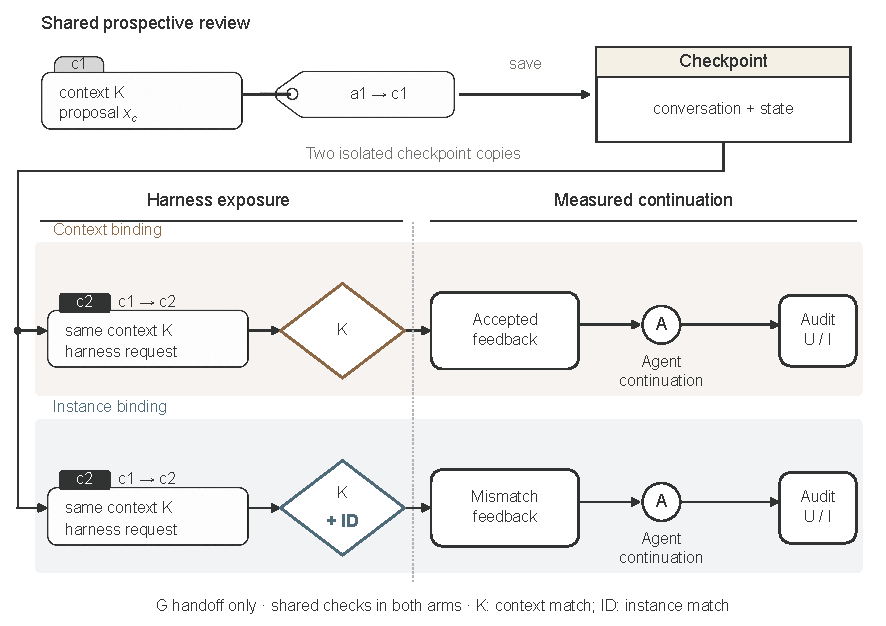
\includegraphics[width=\linewidth]{figures/fig4-paired-intervention.pdf}
\caption{At standardized G handoffs, paired gates differ only in instance equality. The reviewed candidate c1 and its authorization a1 are saved with the conversation and state, then copied into two isolated, directly labelled policy arms. The harness submits c2 with the same context and a different identifier. K denotes $K_{\mathrm{eq}}$; the instance gate adds ID, denoting $I_{\mathrm{eq}}$, while all other checks are shared. Both admission and rejection produce actual feedback for the next sampled agent decision (A), followed by an independent $U/I$ audit. A rejected request makes no commit but leaves the continuation active; subsequent requests must still pass their arm's gate. Measured G outcomes cover 32 delivered pairs from 16 task definitions. N leaves preview management to the agent and is not depicted. Object glyphs were AI-generated; see the AI-assisted preparation declaration}
\label{fig:paired}
\end{figure}


At the queued handoff (G), the harness submits a standardized context-equivalent substitute, after which actual gate feedback enters the next agent decision. The refreshed-preview family (N) leaves management of a required refreshed preview to the agent. Receipt unavailability (R) makes the first receipt query unavailable after a successful commit response has already been delivered; it covers only this confirmed-commit path, and unknown-outcome recovery is a separate deterministic probe (Online Resource 2, A3).

The design separates exposure from behavior. At G, the harness creates and submits the substitute; context admission and the resulting \(I=0\) follow from the policy and oracle definitions, so the 17 and 15 substitution counts are exposure counts rather than agent actions. The behavioral observations begin with the delivered outcome: whether context arms complete, which legal route bound arms choose, their action sequence through the first persistent recovery commit, and any subsequent confirmation calls.

The online host is a separate reduced implementation shared by A and B, not the relational gate of Section \ref{realization-and-external-comparison}. Tasks commit one field and record its source as the successor transition identifier, exercising reduced P5/P6. Controlled implementations test multi-field successors, deep source chains and the full evidence graph. With deterministic grants for valid candidates, reauthorization measures agent routing rather than human review burden.

Configuration A requests \texttt{gpt-5.6-terra} through Codex CLI 0.160.1 with low reasoning; no returned model identifier is exposed. B requests and receives \texttt{deepseek-v4-flash} through an Anthropic-compatible Messages API at temperature zero. Both use the same execution system. Each suffix permits 20 decisions and 24 tool calls, with a 90-second request timeout and a 720-second suffix limit. One format-repair allowance applies across the full prefix-plus-suffix history. B has a 4,096-token response cap; A's upstream cap is unavailable. Frozen inputs and complete settings are in Online Resource 1.

\textbf{Collection provenance.} A provider quota prevented 117 original A pairs from receiving any model response before review. Those previously unexposed pairs form a separately frozen supplementary A collection of 234 arms, retaining task definitions, prompts, tools, policy ordering, requested configuration and scoring. Original outcomes remain unchanged; the later, selected collection has its own denominator and exploratory analysis.

The independent oracle scores utility \(U\) from authoritative goal attainment, required workflow and accurate final reporting. Integrity \(I\) is 1 with sufficient coverage and no contract violation. A proved violation yields 0, and incomplete necessary evidence yields unknown unless a violation is already proved. With no authoritative transition, integrity can hold vacuously and carries no evidence about contract conformance. The instance-continuity oracle applies to both policies, so a context-admissible substitution can score \(I=0\): \(I=0\) records non-conformance to the declared instance rule, not a safety failure under the context rule that the arm declares. Admissibility under a policy and conformity to the independent oracle are different judgments.

For aggregate completion differences, each task contributes the mean of its configuration-specific paired differences (bound minus context). We bootstrap 128 task clusters within family, retaining both policies and configurations (10,000 iterations, seed 20261007). We apply the same procedure separately to the 117 supplementary pairs. Recovery summaries condition on feedback in a saved model input followed by a received response. Recovery calls run from that feedback through the first successful commit that adds a persistent transition; subsequent calls are counted separately. Complete-suffix cost remains the bound-minus-context difference over both full continuations.

\subsection{Task success hides substitution}\label{continuity-and-task-completion}

Substitutions that context binding admits mostly complete their tasks. All proved substitutions occur at G under context binding: 17 in the original collection and 15 in supplementary A. Thirty of these 32 arms still complete their task, so an audit of endpoint utility alone would accept them; the continuity oracle separates them. The 32 episodes come from 16 G task definitions, each observed under deployments B and A. The corresponding bound arms reject the substituted request and all finish with \(U=1,I=1\). Table \ref{tab:outcomes} retains complete cohort denominators, including quota failures and unknown integrity; family-level joint outcomes are in Online Resource 1, S11--S12.

\begin{table}[tbp]
\caption{Completion and instance substitution by collection. Context (Ctx) and instance (Inst; archived as bound) counts are separate; completion denominators remain the planned pairs.}\label{tab:outcomes}
\centering\small
\setlength{\tabcolsep}{2pt}
\begin{tabular*}{\textwidth}{@{\extracolsep{\fill}}lrrrrrrrr@{}}
\toprule
Collection & \shortstack{Planned\\pairs} & \shortstack{Recorded\\checkpoints} & \multicolumn{2}{c}{Completion} & \multicolumn{2}{c}{Substitutions} & \multicolumn{2}{c}{$I$ unknown} \\
\cmidrule(lr){4-5}\cmidrule(lr){6-7}\cmidrule(lr){8-9}
 & & & Ctx & Inst & Ctx & Inst & Ctx & Inst \\
\midrule
Original A & 128 & 11 & 9 & 9 & 1 & 0 & 0 & 0 \\
Original B & 128 & 127\textsuperscript{a} & 117 & 119 & 16 & 0 & 1 & 1 \\
Supplementary A & 117 & 117 & 114 & 116 & 15 & 0 & 0 & 0 \\
\bottomrule
\end{tabular*}
\par\smallskip\begin{minipage}{\textwidth}\small Recorded checkpoints count pairs whose frozen ledger explicitly records reaching the shared review checkpoint. Original A includes 117 pairs stopped by quota before review; supplementary A evaluates those pairs later. \textsuperscript{a}Original B also has one partially recorded N pair without that ledger flag: its context arm retains a partial after-state and its bound arm was not started. It is not reclassified as failing to reach review. These are the two unknown arms. $I$ denotes the independent instance-rule conformance score; arms without an authoritative transition can satisfy it vacuously.\end{minipage}
\end{table}


Observed completion rates are close under the two policies. Across the original collection, completion is 126/256 versus 128/256: +0.78 percentage points, with a 95\% task-cluster interval of {[}−1.95, 3.52{]}. This pooled estimate is dominated by deployment B: original A contributes 11 reviewed pairs and no completion discordance, so the pooled difference is approximately half of the B-specific difference (+1.56 points {[}−3.91, 7.03{]} in original B). The supplementary difference is +1.71 points {[}0.00, 4.27{]}. Neither comparison establishes a completion advantage (Section \ref{threats-to-validity}). Original B has 18 capped invalid-output terminations (10 context, 8 bound); this imbalance constrains interpretation of the original-B completion difference.

A later 24-task output-budget check gives context/bound completion of 23/24 versus 22/24 at 4,096 tokens, and 24/24 for both at 393,216 tokens. Integrity remains 20/24 versus 24/24 at both caps, including four programmed context substitutions per cap. This 96-continuation study uses a later collection period and longer waits; its full results and the original failure decomposition are in Online Resource 2, A1--A2.

\subsection{Two routes to accountable recovery}\label{two-routes-to-accountable-recovery}

All 32 delivered G-bound mismatches recover. Original B's 16 continuations reuse the reviewed candidate; supplementary A has eight reuse and seven reauthorization paths; original A's single mismatch also uses reauthorization. Agents thus select different legal continuations under the same admission rule (Figure \ref{fig:recovery}).

\begin{figure}[tbp]
\centering
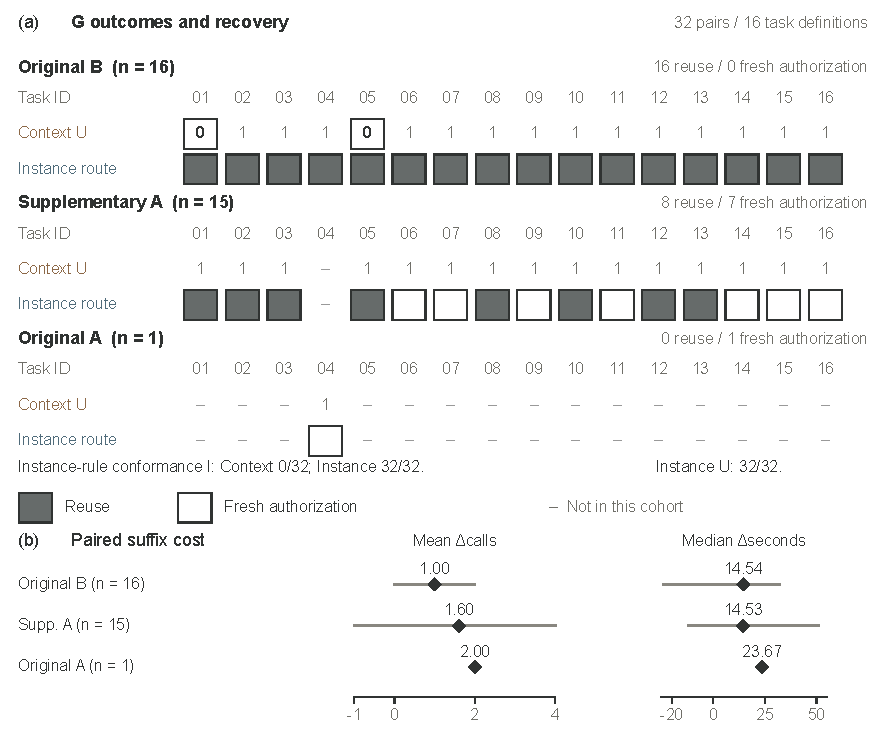
\includegraphics[width=\linewidth]{figures/fig5-recovery-cost.pdf}
\caption{All 32 delivered G pairs across 16 task definitions. (a) Task columns align across cohorts; dashes mean absent from that cohort's delivered pairs, not failure. Supplementary A omits 04; Original A includes only 04. $I$ denotes instance-rule conformance, not safety under the context policy. Context has $I=0$ throughout and $U=1$ in 30 pairs; all bound arms end with $U=1,I=1$. Filled/open squares denote reuse/fresh authorization. (b) Diamonds show mean call and median elapsed-time differences for complete paired suffixes ($\Delta=$ bound minus context); segments show observed minima--maxima, not confidence intervals. Time includes decisions, tool interactions and terminal paths. Table~\ref{tab:recovery-decomposition} separates recovery calls}
\label{fig:recovery}
\end{figure}


The observed recovery sequences are direct. After delivered feedback, each of the 24 reuse episodes makes one commit, and each of the eight fresh-authorization episodes requests authorization and then commits. No failed or exploratory tool call intervenes before these successful recovery commits. Later receipt or state queries are separate continuation actions (Table~\ref{tab:recovery-decomposition}). The measurements cover agent continuation under the tested interface with immediate deterministic authorization.

An archived example makes the interface dependence explicit. In original-B pair \texttt{FORMAL-G-002-B}, the saved review response already supplies candidate \texttt{c1}, grant \texttt{a1} and authorized value 3412. The harness submits \texttt{c2} and returns \texttt{INSTANCE\_MISMATCH}; the next agent action commits \texttt{c1} under \texttt{a1}, creating one transition. A later \texttt{get\_receipt} call confirms that commit without another transition. Thus this episode contributes one recovery call and one subsequent confirmation call, versus zero agent calls in its context suffix. The saved feedback does not select a recovery route for the agent. Online Resource 1, S12.6 gives the event and state anchors.

\begin{table}[tbp]
\caption{Agent tool calls at delivered G handoffs. All entries except $n$ are cohort means; post-commit calls occur after the first successful persistent recovery commit.}\label{tab:recovery-decomposition}
\centering\small
\setlength{\tabcolsep}{3pt}
\begin{tabular*}{\textwidth}{@{\extracolsep{\fill}}lrrrrrr@{}}
\toprule
Collection & $n$ & \shortstack{To recovery\\commit} & \shortstack{After\\commit} & \shortstack{Bound\\suffix} & \shortstack{Context\\suffix} & $\Delta$ \\
\midrule
Original A & 1 & 2.000 & 2.000 & 4.000 & 2.000 & 2.000 \\
Original B & 16 & 1.000 & 0.375 & 1.375 & 0.375 & 1.000 \\
Supplementary A & 15 & 1.467 & 1.533 & 3.000 & 1.400 & 1.600 \\
\bottomrule
\end{tabular*}
\par\smallskip\begin{minipage}{\textwidth}\small Recovery comprises one commit in each of 24 reuse episodes and an authorization request followed by a commit in each of eight fresh-authorization episodes. The last column is bound minus context over complete suffixes, not calls beyond a route minimum. Values are recomputed from the archived event order and persistent transitions; no new runs are added.\end{minipage}
\end{table}


Complete paired suffixes add a mean 1.00 tool call and median 14.54 seconds in original B, versus 1.60 calls and 14.53 seconds in supplementary A. The latter's seven reauthorization paths average 0.47 authorization requests across 15 pairs. Original A's single pair adds two calls and 23.67 seconds. Table~\ref{tab:recovery-decomposition} separates recovery, subsequent and context-side calls; Figure~\ref{fig:recovery} preserves signed ranges. E/V/R delivered-episode results remain separate in Online Resource 1, S11--S12.

\subsection{Exposure without rejection feedback}\label{opportunity-and-voluntary-behavior}

Agents shown a context-equivalent alternative reused the reviewed instance or obtained fresh authorization. The N family supplies such an alternative without forcing its submission. Across the collections, 186 arms were planned, 185 retain state and 127 reached review. Of these, 124 received a preview of a different-identity, same-context candidate in a saved model input, followed by a non-error response; these are arm-level exposures, and the two policy arms of a task share one prefix. Agents reused the reviewed instance in 123 cases and obtained matching authorization for the previewed candidate in one; there were zero unauthorized substitutions.

One original-B context arm supports only observation through its saved after-state, and its bound counterpart was not started; both integrity scores remain unknown. Excluding the partial arm leaves 126 reviewed arms, 123 exposures, 122 reuses and one reauthorization (Online Resource 2, A7). N thus shows two continuity-preserving behaviors when an alternative is available. G measures recovery from delivered mismatch feedback; N contains no such feedback.

\section{Discussion}\label{discussion}

\subsection{Implications}\label{design-implications}

Approval scope and continuation must be designed together. Context or content binding permits declared equivalences; instance binding turns a replacement into a rejection requiring agent action. The observed reuse, reauthorization and later confirmation show why a builder must specify both the allowed replacement and the interface for continuing after rejection.

These results suggest four choices for builders:
\begin{enumerate}
\tightlist
\item \textbf{Obtain the responsibility rule.} Have the workflow owner state whether approval covers a value, retained context, declared content or the reviewed artifact, and which replacements may reuse it. The measurements do not decide this organizational requirement.
\item \textbf{Cover the reusable content.} Put each decision-relevant field in the reuse key or check its approved value separately at execution; declare the comparator.
\item \textbf{Anchor binding and recovery.} Resolve identifiers through trusted lookup to immutable candidates; return the reviewed identifier or the state/evidence mismatch needed for reuse or fresh authorization. A valid original grant can support reuse even for an irreversible operation; stale state or evidence can require fresh authorization even for a reversible one.
\item \textbf{Check external objects at consumption.} Verify the reviewed digest and execute on the same captured bytes, as in the tested adapter.
\end{enumerate}

The ToolGate adaptation illustrates this separation: framework callbacks express the obligations, while the application bridge supplies durable enforcement.

\subsection{Threats to validity}\label{threats-to-validity}

\textbf{Construct validity.} Measured costs are agent-side tool calls and suffix time. Gate computation was not isolated; human re-inspection and approval-queue waiting were not measured. The deterministic reviewer immediately grants any valid request, whereas a deployed reauthorization request may wait, be refused or require transfer to an authorized reviewer. The observed routes and suffix times do not establish optimal route selection or production approval latency. Canonical equality is enforced at the gate; agreement between displayed and compared values was tested only in the browser fixture. The binding-scope study implements the selected comparators and a common executor, not the complete set of shared checks \(G\), and normalizes money to two decimals instead of canonical JSON equality.

\textbf{Internal validity.} G substitutions are harness-created exposures (Section \ref{design-and-measurement}), and each cell has one realization. G recovery and N continuation were observed under the common preview--authorization instruction, with an additional reminder in N; no control without warnings isolates these prompts' effects. The completion comparisons are not powered for a non-inferiority claim, and an interval that includes zero does not establish equivalence. The supplementary cohort and the output-budget study retain separate collection conditions and denominators. The deterministic protocol was amended after inspecting an initial run, and its 72 routes are crossed conditions over nine constructed cases, not independent samples.

\textbf{External validity.} Tasks are constructed, the reviewer is deterministic and the online host exercises a reduced single-field form of the contract. Natural mismatch prevalence, human approval cost and production benefit remain open empirical questions. The ToolGate comparison uses scripted decisions and an author-written commit bridge; it does not measure native default admission, autonomous agent performance or an efficiency advantage. The native-default study uses an in-process checkpointer and does not test restarts, concurrent replay or unauthorized post-approval mutation. Beyond the deterministic binding comparison, only two points of the design space are tested with agents; the remaining combinations have not been validated in a developer study.

\textbf{Scope of the formal results.} The formal and persistence results apply to the stated local observation model and atomic single-record successor (Section \ref{what-endpoint-correctness-cannot-establish}); multi-record or distributed enforcement requires additional coordination.

\section{Conclusion}\label{conclusion}

An approval's binding object determines which replacements it permits. The four-role correction contract connects this choice to authorized values, successor structure and field sources. Constructed comparisons, store realizations and a ToolGate adaptation make the obligations executable; paired identity-only handoffs reveal reuse and reauthorization, with confirmation costs accounted for separately. Together, they support implementing a declared approval scope at the write boundary with a corresponding recovery interface.